\subsection{Chapter 15 - Electric charges and fields}

\subsubsection{Overview}\label{chapter:chargesfields}

In this and subsequent chapters, we start to look at the theories that describe electric and magnetic phenomena. Within the framework for dynamics that was developed by Newton, we will introduce the theories of electromagnetism which describe the electric force, the magnetic force, and how these two interact. This first chapter introduces the description of the electric force, analogously to how we introduced Newton's Universal Theory of Gravity to describe the gravitational force.

\begin{framed}
\textbf{Learning Objectives}\\
\begin{itemize}
\item Understand the definition of an electric charge.
\item Understand the difference between an insulator and a conductor.
\item Understand different mechanisms for charging objects.
\item Understand Coulomb's model for the electric force.
\item Understand the definition of an electric field.
\item Understand how to calculate the electric field from a continuous distribution of charge.
\item Understand how to model an electric dipole.
\end{itemize}
\end{framed}

\begin{framed}
\textbf{Think About It}\\
If you rub a balloon against a carpet and bring it near your head, your hair will stand up and try to touch the balloon.

\begin{enumerate}
\item The electric charge of the balloon is opposite of that on your hair.
\item Your hair has no net electric charge, this is an example of charge separation and induction.
\end{enumerate}

\begin{framed}
\textbf{Answer}\\
\begin{enumerate}[resume]
\item
\end{enumerate}
\end{framed}
\end{framed}

\subsubsection{Electric charge}

You have likely experienced or heard about electric charge in your life. For example, on a dry winter day, you might find that after rubbing your bare feet on a polyester carpet, you feel a small electric shock upon touching a metallic surface such as a doorknob. You probably also know that there are positive and negative charges, and that equal charges repel each other whereas opposite charges attract. In this chapter, we develop the description of how these charges can accumulate and how they exert attractive or repulsive forces on each other.

Ordinary matter is made of atoms, which are themselves made of a small positive nucleus (containing positive protons and neutral neutrons) surrounded by a ``cloud'' of negatively charged electrons. Within a solid object, inter-atomic forces hold the atoms together, so we can model the atoms as being effectively stationary. This means that we can treat the positive nuclei as being fixed in space. The negative electrons, depending on the material, can often move from one atom to another. If an atom loses an electron to another atom, it becomes positive, whereas the atom that acquired the extra electron becomes negative.

We define the net charge on an atom (or an object) based on whether there are more protons (positive), more electrons (negative) or an equal amount (neutral). By default, atoms are neutral and have an equal number of protons and electrons. An object becomes charged when it acquires an excess (or deficit) of electrons from another object. We say that ``charge is conserved'' because the number of electrons in the system does not change, i.e. if one object became positively charged, a different object must have become negatively charged by the same amount, so that the total net charge (in the Universe) is zero.

When you rub two objects together, you allow electrons to be transferred between them. Different materials have different ``affinities'' for electrons, and the electrons will transfer to the object with the highest affinity. Returning to our earlier example, when you rub your bare feet on the polyester carpet, electrons are being removed from your feet and deposited onto the carpet. Since your feet lose electrons, you acquire a net positive charge, while the carpet acquires a net negative charge. This way of creating a net charge on an object is called ``charging by friction''. If you then touch a doorknob, electrons will jump from the doorknob and onto your (now positively charged) body, creating a spark.

The ``triboelectic series'' is a list of materials that tend to give up or acquire electrons when they are placed in close contact with each other. Some common materials from the series are shown in Figure~\ref{fig:chargesfields:triboseries}.  The greatest charge is generated by rubbing together materials that are the furthest apart from each other in the diagram. Rubbing silk on a piece of glass results in more charge than rubbing wool on the same piece of glass.

\begin{figure}[!htbp]
\centering
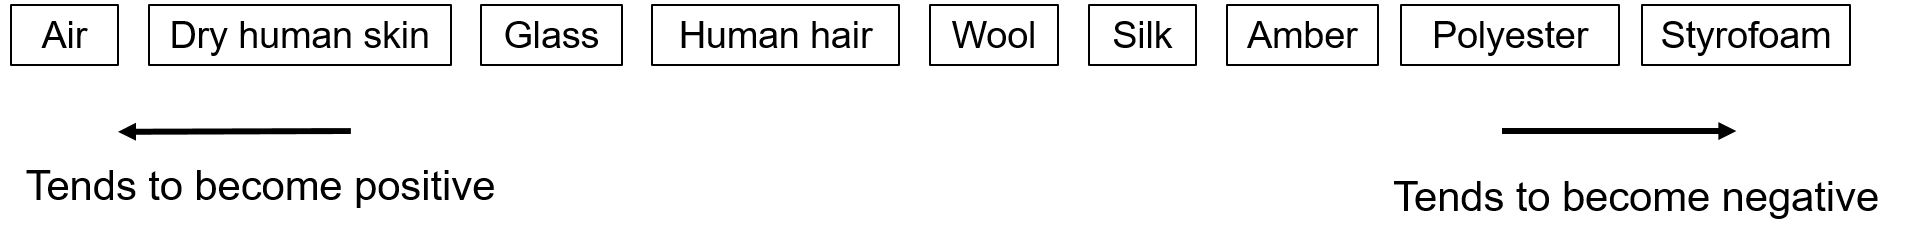
\includegraphics[width=1\linewidth]{files/triboseries-4b056b04414ba5a33d35300655cca63b.png}
\caption[]{A sample of a triboelectric series of materials. The materials on the right-hand side have the greatest affinity to acquire electrons.}
\label{fig:chargesfields:triboseries}
\end{figure}

\begin{framed}
\textbf{Checkpoint}\\
If you rub a glass rod with silk, which object ends up with an excess of electrons?\}

\begin{enumerate}
\item glass rod.
\item silk.
\item neither, they remain neutral.
\item both will acquire an excess of electrons.
\end{enumerate}

\begin{framed}
\textbf{Answer}\\
\begin{enumerate}[resume]
\item
\end{enumerate}
\end{framed}
\end{framed}

\paragraph{Conductors and insulators}

We can broadly classify materials into conductors (such as metals), and insulators (such as wood), depending on how easily the electrons can move around in the material. In a conductor, electrons (rather, the outer electron(s) of an atom) are only loosely bound to their nuclei, and they can thus move around the material freely. In an insulator, the electrons are tightly bound to the nuclei of their atoms and cannot easily move around. There is a third class of materials, semi-conductors, that falls somewhere between a conductor and an insulator. In a semi-conductor, electrons are typically bound to their atoms, but any additional electrons present in the material can move around as if they are in a conductor.

Within a conductor, such as a solid metallic sphere, charges can move around freely. If that sphere has a net charge, for example an excess of electrons, those excess electrons will migrate to the outer surface of the sphere. Electrons in the sphere repel each other and will quickly settle into a position where they are, on average, the furthest from all of the other electrons, which occurs if all of the electrons migrate to the surface. This is illustrated in the left panel of Figure~\ref{fig:chargesfields:conductioncharge}. If an initially neutral conducting sphere is connected to the charged sphere by a conducting wire (right panel of Figure~\ref{fig:chargesfields:conductioncharge}), some of the electrons will ``conduct'' (transfer) onto the surface of the neutral sphere, so that, on average, they are further from all other electrons. This way of adding charge to the neutral sphere is called ``charging by conduction'', and the second sphere will remain charged if the connection between spheres is broken.

\begin{figure}[!htbp]
\centering
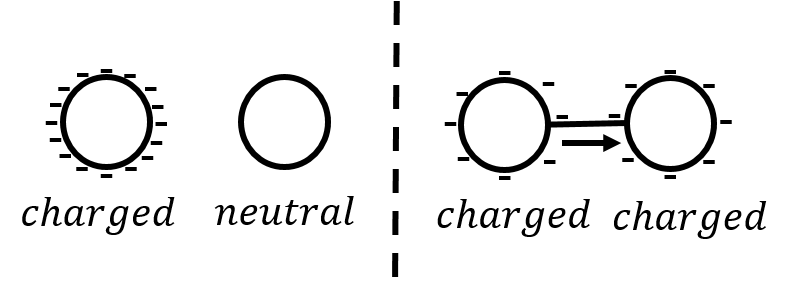
\includegraphics[width=0.7\linewidth]{files/conductioncharge-13c1ad8aca42859d6e0e2273eeb697c0.png}
\caption[]{Charging by conduction: a neutral conducting sphere is connected to a negatively charged conducting sphere. The charges can ``spread out more'' if some of the charges move (``conduct'') from the charge sphere onto the neutral sphere.}
\label{fig:chargesfields:conductioncharge}
\end{figure}

\paragraph{Electrostatic induction}

Electrostatic induction allows one to ``induce'' a charge by using the fact that charges can move freely in a conductor. The left panel of Figure~\ref{fig:chargesfields:induction} shows a (neutral) rod made of a conducting material, with electrons distributed uniformly throughout its volume. In the right panel, a negatively charged sphere is brought next to the rod. The negative sphere repels the electrons in the rod. Since the rod is conducting, the electrons can move around easily, and so they move to the end of the rod that is furthest from the negative sphere. Those electrons will leave positive charges (corresponding to the atoms that have lost their electrons) on the side closest to the sphere. The electrons in the rod will only accumulate for as long as the force from the negative sphere is greater than the repulsive force from the electrons that have already accumulated. In practice, such an equilibrium is reached almost instantly. In equilibrium, we say that the rod is ``polarized'', or that the ``charges in the rod have separated'', although the rod is overall still neutral.

Note that we can model this as if it where positive charges that move inside of the rod instead of negative charges. The positive charges are attracted to the negative sphere, and thus accumulate on the end of the rod closest to the sphere, leaving a negative charge on the other end. The choice to call electrons ``negative'' is completely arbitrary. For convenience, we usually build models assuming that positive charges can easily move around, even if, in reality, it is almost always actually (negative) electrons that move.

\begin{figure}[!htbp]
\centering
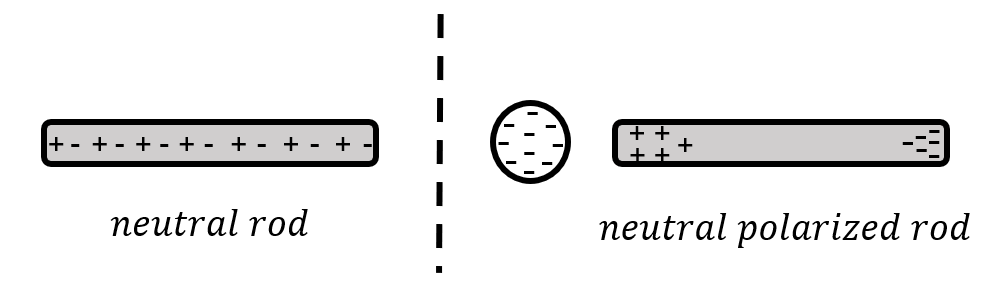
\includegraphics[width=0.9\linewidth]{files/induction-61f57859342bff8910b8621b0315b66b.png}
\caption[]{Electrostatic induction: when a negatively charged sphere is brought close to a neutral conducting rod, the electrons in the rod, which can move freely, accumulate on the side of the rod furthest from the sphere, leaving an excess of positive charge near the sphere.}
\label{fig:chargesfields:induction}
\end{figure}

We can create a net charge on the polarized rod if we provide a conducting path for charges to leave (or enter) the rod. The Earth can be modelled as a very large reservoir of both positive and negative charges. By connecting the rod to the Earth (we say that we connect the rod to ``ground''), we provide a path for the electrons in the rod to be even further from the negatively charged sphere, and they can thus leave the rod entirely in order to go into the ground. This is illustrated in the right-hand panel of Figure~\ref{fig:chargesfields:inductioncharge}.

If we then disconnect the rod from the ground, it has now acquired an overall positive charge, as in the right hand panel. We call this ``charging by induction''. We can also think of this in terms of positive charges moving into the rod from the Earth; when we connect the rod to the ground, the positive charges in the Earth can move into the rod and get closer to the negatively charged sphere. If we disconnect the rod from the ground, the rod stays positive, just as we conclude when using a model where it is the negative charges that move\footnote{Unless magnetism is involved, it is not possible to distinguish between a flow of positive charges moving in one direction or negative charges moving in the opposite direction.
[\^41\};Others had initially observed the inverse square law for the electric force, but Coulomb was the first to formalize the theory.}.

\begin{figure}[!htbp]
\centering
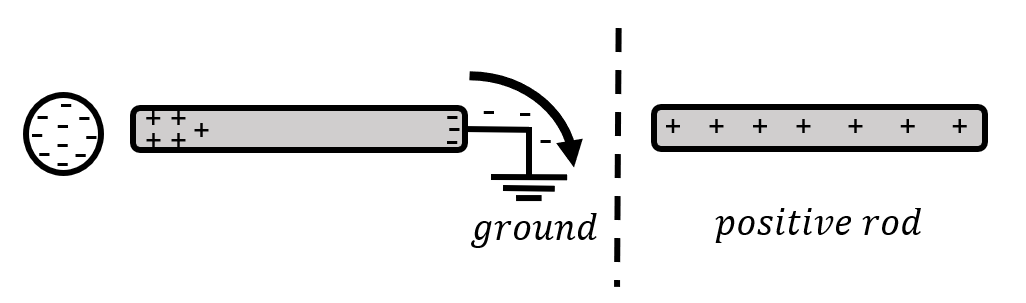
\includegraphics[width=0.9\linewidth]{files/inductioncharge-7664b6a2f86d0f9e6767bf0ce16ca03e.png}
\caption[]{Charging by induction: when we connect the polarized rod to the ground, electrons can leave the rod. If we now disconnect the rod from ground, the rod is left with an overall positive charge.}
\label{fig:chargesfields:inductioncharge}
\end{figure}

\begin{framed}
\textbf{Olivia's Thoughts}\\
Before we leave this section, let's take a minute to summarize the different methods for charging an object.

\begin{enumerate}
\item Charging by friction: We start with two neutral objects. To charge the objects, we rub them together. We end up with two oppositely charged objects. To explain this, we need to know that atoms can exchange electrons when they are in close contact and that different materials have different affinities for electrons.
\item Charging by conduction: We start with one neutral object and one charged object. To charge the neutral object, we put it in contact with the charged object. Charges move from the charged object to the neutral object, so we end up with two objects that are both positive or both negative. To explain this, we need to know that like charges repel, and that charges can move around freely inside conductors.
\item Charging by induction: We start with one neutral object and one charged object. To charge the neutral object, we move the charged object close to (but not touching) the neutral object to separate the charges in the neutral object. We then use some mechanism (e.g. connecting to ground) to create a net charge. We end up with one positively charged object and one negatively charged object. Once again, we need to know that like charges repel, and that charges can move around freely in conductors.
\end{enumerate}
\end{framed}

\subsubsection{The Coulomb force}

Coulomb was the first to provide a detailed quantitative description of the force between charged objects. Nowadays, we use the (derived) SI unit of ``Coulomb'' (C) to represent charge. The ``charge'' of an object corresponds to the net excess (or lack) of electrons on the object. An electron has a charge of $-e= -1.6\times 10^{ -19} {\rm C}$. Thus, an object with a charge of $-1 {\rm C}$ has an excess of about $\frac{1}{1.6\times 10^{ -19}}=6.25\times 10^{18}$ electrons on it, which is a very large charge. If an object has an excess of electrons, it is negatively charged and we indicate this with a negative sign on the charge of the object. An object with a (positive) charge of $1 {\rm C}$ thus has a deficit of $6.25\times 10^{18}$ electrons.

Through careful studies of the force between two charged spheres, Coulomb observed[\^41] that:

\begin{itemize}
\item The force is attractive if the objects have opposite charges and repulsive if the objects have the same charge.
\item The force is inversely proportional to the squared distance between spheres.
\item The force is larger if the charges involved are larger.
\end{itemize}

This leads to Coulomb's Law for the electric force (or simply ``Coulomb's Law''), $\vec F_{12}$, exerted on a point charge $Q_1$ by another point charge $Q_2$:
\begin{equation}
\boxed{\vec F_{12}=k\frac{Q_1Q_2}{r^2}\hat r_{21}}
\end{equation}
where $\hat r_{21}$ is the unit vector from $Q_2$ to $Q_1$ and $r$ is the distance between the two charges, as illustrated in Figure~\ref{fig:chargesfields:coulombforce}. Coulomb's constant, $k=8.99\times 10^9 {\rm N\cdot m^2/C^{2}}$, is simply a proportionality constant to ensure that the quantity on the right will have units of Newtons when all other quantities are in S.I. units. In some instances, it is more convenient to use the ``permittivity of free space'', $\epsilon_0$, rather than Coulomb's constant, in which case Coulomb's Law has the form:
\begin{equation}
\vec F_{12}=\frac{1}{4\pi\epsilon_0}\frac{Q_1Q_2}{r^2}\hat r_{21}
\end{equation}
where $\epsilon_0=\frac{1}{4\pi k}=8.85\times 10^{ -12} {\rm C^2\cdot N^{ -1}\cdot m^{ -2}}$ is a more fundamental constant, as we will see in later chapters.

\begin{figure}[!htbp]
\centering
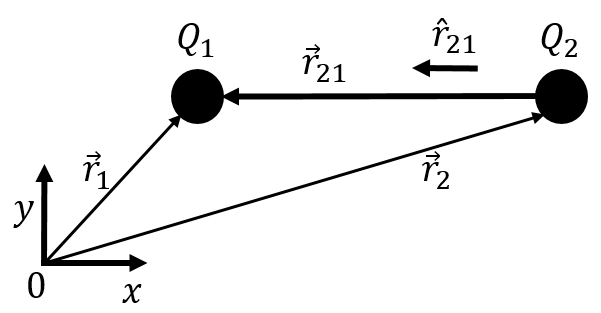
\includegraphics[width=0.5\linewidth]{files/coulombforce-596abbc328557b381fefd6d5708cb366.png}
\caption[]{Vectors involved in applying Coulomb's Law.}
\label{fig:chargesfields:coulombforce}
\end{figure}

If the two charges have positions $\vec r_1$ and $\vec r_2$, respectively, then the vector $\hat r_{21}$ is given by:
\begin{equation}
\hat r_{21} = \frac{\vec r_2 - \vec r_1}{||\vec r_2 - \vec r_1||}
\end{equation}
Coulomb's Law is mathematically identical to the gravitational force in Newton's Universal Theory of Gravity. Rather than quantity of mass determining the strength of the gravitational force, it is the quantity of charge that determines the strength of the electric force. The only major difference is that gravity is always attractive, whereas the Coulomb force can be repulsive.

\begin{framed}
\textbf{Checkpoint}\\
The Coulomb force is conservative.

\begin{enumerate}
\item True.
\item False.
\end{enumerate}

\begin{framed}
\textbf{Answer}\\
\begin{enumerate}
\item
\end{enumerate}
\end{framed}
\end{framed}

The product $Q_1Q_2$ in the numerator of Coulomb's force is positive if the two charges have the same sign (both positive or both negative) and negative if the charges have opposite signs. Again, referring to Figure~\ref{fig:chargesfields:coulombforce}, if the two charges are positive, the force on $Q_1$ will point in the same direction as $\hat r_{21}$ (since all of the scalars are positive in Coulomb's Law) and thus be repulsive. If, instead, the two charges have opposite signs, the product $Q_1Q_2$ will be negative and the force vector on $Q_1$ will point in the opposite direction from $\hat r_{21}$ and the force is attractive.

\begin{framed}
\textbf{Example 15.1}\\
Calculate the magnitude of the electric force between the electron and the proton in a hydrogen atom and compare this to the gravitational force between them.

\begin{framed}
\textbf{Solution}\\
We model this by assuming that the electron and proton are point charges a distance of $1 \overset{\circ}{\rm A}=1\times 10^{ -10} {\rm m}$ apart (1 Angstrom is about the size of the hydrogen atom). The proton and electron have the same charge with magnitude $e=1.6\times 10^{ -19} {\rm C}$, so the (attractive) electric force between them has a magnitude of:
\begin{equation}
F_e &= k\frac{Q_1Q_2}{r^2}\\
&=(9\times 10^9 {\rm N\cdot m^2/C^{2}})\frac{(1.6\times 10^{-19} {\rm C})(1.6\times 10^{-19} {\rm C})}{(1\times 10^{-10} {\rm m})^2}\\
&=2.3\times 10^{-8} {\rm N}
\end{equation}
which is a small number, but acting on a very small mass. In comparison, the force of gravity between an electron ($m_e=9.1\times 10^{ -31} {\rm kg}$) and a proton ($m_p=1.7\times 10^{ -27} {\rm kg}$) is given by:
\begin{equation}
F_g&=G\frac{m_em_p}{r^2}\\
&=(6.7\times 10^{-11} {\rm Nm^2/kg^2})\frac{(9.1\times 10^{-31} {\rm kg})(1.7\times 10^{-27} {\rm kg})}{(1\times 10^{-10} {\rm m})^2}\\
&=1.04\times 10^{-47} {\rm N}
\end{equation}
\textbf{Discussion:} As we can see, the electric force between an electron and a proton is 39 orders of magnitude larger than the gravitational force! This shows that the gravitational force is extremely weak on the scale of particles and has essentially no effect in particle physics. Indeed, the best current theory of particle physics, and the most precisely tested theory in physics, the ``Standard Model'', does not need to include gravity in order to provide a spectacularly precise description of particles. One of the big challenges in theoretical physics is nonetheless to develop a theory that integrates the gravitational force with the other forces.
\end{framed}
\end{framed}

In the following trinket, a positive and negative charge are drawn. The force each charge experiences is drawn as an arrow and calculated for a distance of $1 \overset{\circ}{\rm A}=1\times 10^{ -10} {\rm m}$ apart. Following convention, the vector arrows have their origin at the charge experiencing the force. When the trinket is run, the force arrows indicate an attractive force, i.e., the charges experience forces toward one another. If the charges are changed to like charges, e.g., \texttt{Q1.q = q} and \texttt{Q2.q = q}, the force arrows indicate repulsion between the charges.

\begin{figure}[!htbp]
\centering
\caption[]{A trinket demonstrating Coulomb Force between opposite charges.}
\label{chap:chargesfields:coulombtrinket}
\end{figure}

\begin{framed}
\textbf{Example 15.2}\\
Three charges, $Q_1=1 {\rm nC}$, $Q_2= -2 {\rm nC}$, and $q= -1 {\rm nC}$, are held fixed at the three corners of an equilateral triangle with sides of length $a=1 {\rm cm}$, with a coordinate system as shown in Figure~\ref{fig:chargesfields:chargetriangle}. What is the electric force vector on charge $q$? (Note that $1 {\rm nC}=1\times 10^{ -9} {\rm C}$).

\begin{figure}[!htbp]
\centering
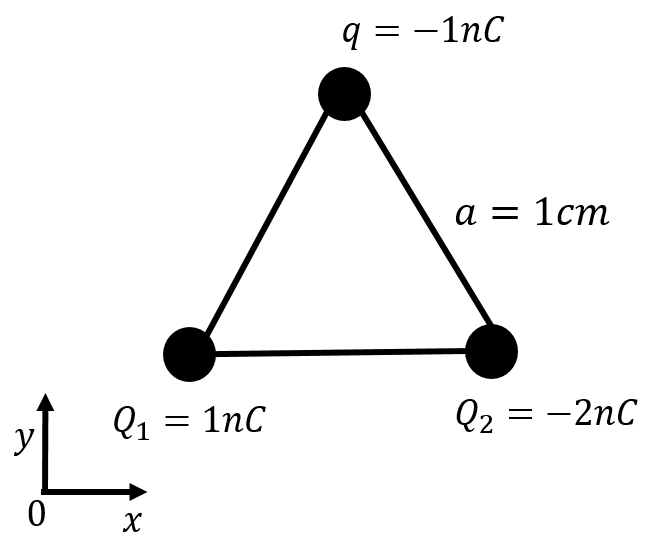
\includegraphics[width=0.4\linewidth]{files/chargetriangle-6c806c6caa350d0b775548735919e542.png}
\caption[]{Three charges arranged in an equilateral triangle of side $a$.}
\label{fig:chargesfields:chargetriangle}
\end{figure}

\begin{framed}
\textbf{Solution}\\
The net electric force on charge $q$ will be the vector sum of the forces from charges $Q_1$ and $Q_2$. We thus need to determine the force vectors on $q$ from each charge using Coulomb's Law, and then add those two vectors to obtain the net force on $q$. The force vectors exerted on $q$ from each charge are illustrated in Figure~\ref{fig:chargesfields:chargetriangle_sol}.

\begin{figure}[!htbp]
\centering
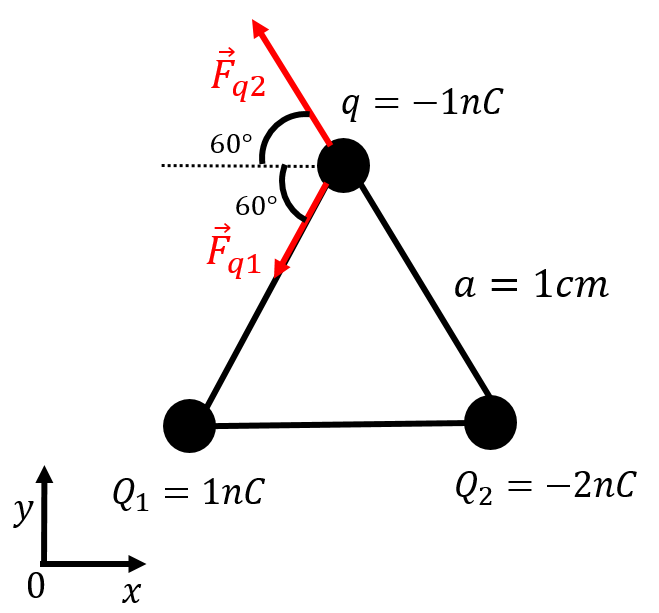
\includegraphics[width=0.4\linewidth]{files/chargetriangle_sol-8952ca5b443a1c0f12a01e7a166f9cfb.png}
\caption[]{Force vectors on charge $q$.}
\label{fig:chargesfields:chargetriangle_sol}
\end{figure}

The force from charge $Q_1$ has magnitude:
\begin{equation}
F_{q1}=\left |k\frac{Q_1q}{a^2}\right |=(9\times 10^9 {\rm N\cdot m^2/C^{2}})\frac{(1\times 10^{-9} {\rm C})(1\times 10^{-9} {\rm C})}{(0.01 {\rm m})^2}=9\times 10^{-5} {\rm N}
\end{equation}
and components:
\begin{equation}
\vec F_{q1}&=-F_{q1}\cos(60 {\rm \degree})\hat x-F_{q1}\sin(60 {\rm \degree})\hat y\\
&=-(4.5\times 10^{-5} {\rm N})\hat x-(7.8\times 10^{-5} {\rm N})\hat y
\end{equation}
Similarly, the force on $q$ from $Q_2$ has magnitude:
\begin{equation}
F_{q2}=\left |k\frac{Q_2q}{a^2}\right |=(9\times 10^9 {\rm N\cdot m^2/C^{2}})\frac{(2\times 10^{-9} {\rm C})(1\times 10^{-9} {\rm C})}{(0.01 {\rm m})^2}=1.8\times 10^{-4} {\rm N}
\end{equation}
and components:
\begin{equation}
\vec F_{q2}&=-F_{q2}\cos(60 {\rm \degree})\hat x+F_{q2}\sin(60 {\rm \degree})\hat y\\
&=-(9.0\times 10^{-5} {\rm N})\hat x+(1.6\times 10^{-4} {\rm N})\hat y
\end{equation}
Finally, we can add the two force vectors together to obtain the net force on $q$:
\begin{equation}
\vec F^{net}&=\vec F_{q1}+\vec F_{q2}\\
&=-(4.5 \times 10^{-5} {\rm N})\hat x-(7.8 \times 10^{-5} {\rm N})\hat y-(9.0 \times 10^{-5} {\rm N})\hat x+(1.6 \times 10^{ 4} {\rm N})\hat y\\
&=-(13.5\times 10^{-5} {\rm N})\hat x+(8.2\times 10^{-5} {\rm N})\hat y
\end{equation}
which has a magnitude of $15.8\times 10^{ -5} {\rm N}$.

\textbf{Discussion:} In this example, we determined the net force on a charge by making use of the superposition principle; namely, that we can treat the forces exerted on $q$ by $Q_1$ and $Q_2$ independently, without needing to consider the fact that $Q_1$ and $Q_2$ exert forces on each other.
\end{framed}
\end{framed}

\subsubsection{The electric field}

We define the electric field vector, $\vec E$, in an analogous way as we defined the gravitational field vector, $\vec g$. By defining the gravitational field vector, say, at the surface of the Earth, we can easily calculate the gravitational force exerted by the Earth on any mass, $m$, without having to use Newton's Universal Theory of Gravity. As you recall, we can define the gravitational field, $\vec g(\vec r)$, at some position, $\vec r$, from a point mass, $M$, as the gravitational force per unit mass:
\begin{equation}
\vec g(\vec r) = -G \frac{M}{r^2}\hat r
\end{equation}
where $\vec r$ is a vector from the position of $M$ to where we want to know the gravitational field. As a result, the force exerted on a ``test mass'', $m$, located at position $\vec r$ relative to mass $M$ is given by:
\begin{equation}
\vec F_g=m\vec g= -G\frac{Mm}{r^2}\hat r
\end{equation}
which, of course, is the result from Newton's Theory of Gravity. As you recall, we can define the gravitational field for  any object that is not a point mass (e.g. the Earth), and use that field to find the force exerted by the Earth on any mass $m$, without having to re-calculate the gravitational field each time (which requires an integral or Gauss' Law).

We proceed in an analogous way to define the ``electric field'', $\vec E(\vec r)$, as the \textit{electric force per unit charge}. If we have a point charge, $Q$, located at the origin of a coordinate system, then the electric field from that point charge, $\vec E(\vec r)$, at some position, $\vec r$, relative to the origin is given by:
\begin{equation}
\boxed{\vec E(\vec r) = k\frac{Q}{r^2}\hat r}
\end{equation}
If we place a ``test charge'', $q$, at position $\vec r$ in space, it will experience a force given by:
\begin{equation}
\vec F_e=q\vec E=k\frac{Qq}{r^2}\hat r
\end{equation}
just as we find from Coulomb's Law.

\begin{framed}
\textbf{Checkpoint}\\
A negative charge is placed at the origin of a coordinate system. At some point in space, the electric field from that charge

\begin{enumerate}
\item points towards the origin.
\item points away from the origin.
\end{enumerate}

\begin{framed}
\textbf{Answer}\\
\begin{enumerate}
\item
\end{enumerate}
\end{framed}
\end{framed}

In Three~charges~arranged~in~an~equilateral~triangle~of~side~a., we determined the electric force on charge $q$, exerted by two other charges $Q_1$ and $Q_2$. If we now changed the value of $q$ and wanted to determine the force, we can use the electric field to simplify the process considerably. That is, we can determine the value of the electric field, $\vec E$, from $Q_1$ and $Q_2$ at the position of $q$, and then simply multiply that field vector by a charge $q$ to obtain the force on that charge, without having to add force vectors.

\begin{framed}
\textbf{Example 15.3}\\
Two charges, $Q_1=1 {\rm nC}$, and $Q_2= -2 {\rm nC}$ are held fixed at two corners of an equilateral triangle with sides of length $a=1 {\rm cm}$, with a coordinate system as shown in Figure~\ref{fig:chargesfields:chargetriangle}. What is the electric field vector at the third corner of the triangle?

\begin{figure}[!htbp]
\centering
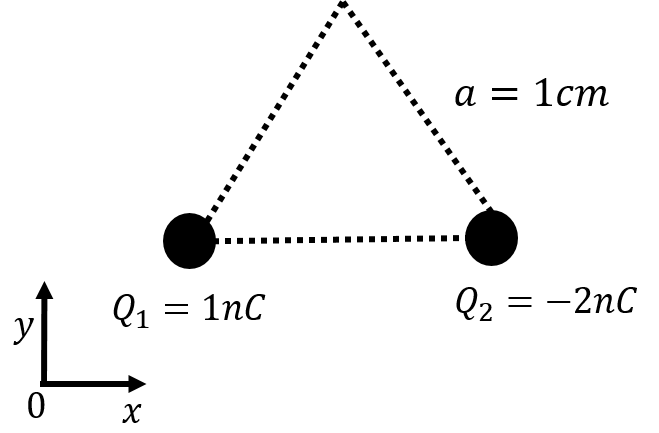
\includegraphics[width=0.4\linewidth]{files/fieldtriangle-c6a57a30ed4678046ce1a02cb4519207.png}
\caption[]{Two charges at the corners of an equilateral triangle of side $a$.}
\label{fig:chargesfields:fieldtriangle}
\end{figure}

\begin{framed}
\textbf{Solution}\\
The net electric field at the third corner of the triangle will be the vector sum of the electric fields from charges $Q_1$ and $Q_2$. We thus need to determine the electric field vectors from each charge, and then add those two vectors to obtain the net electric field. The vectors are illustrated in Figure~\ref{fig:chargesfields:fieldtriangle_sol}.

\begin{figure}[!htbp]
\centering
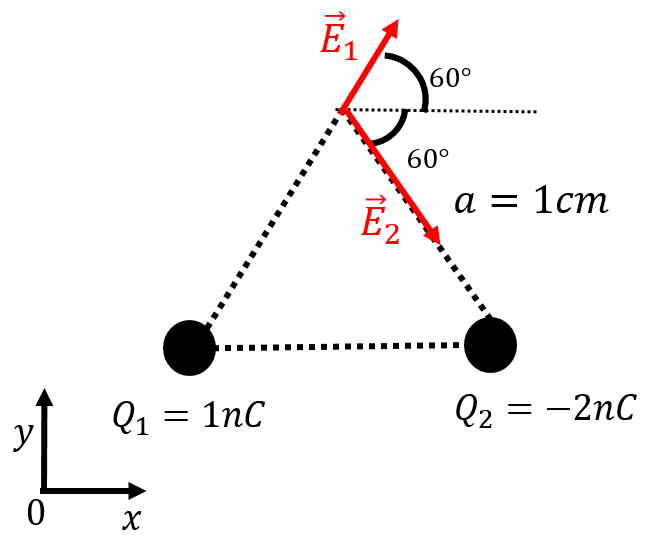
\includegraphics[width=0.4\linewidth]{files/fieldtriangle_sol-d6d26a9828e420c4da7572c93d22e5b3.png}
\caption[]{Electric field vectors from two charges at the corners of an equilateral triangle of side $a$.}
\label{fig:chargesfields:fieldtriangle_sol}
\end{figure}

The electric field from charge $Q_1$ has magnitude:
\begin{equation}
E_1=\left |k\frac{Q_1}{a^2}\right |=(9\times 10^{9} {\rm N\cdot m^2/C^{2}})\frac{(1\times 10^{-9} {\rm C})}{(0.01 {\rm m})^2}=9\times 10^{4} {\rm N/C}
\end{equation}
and components:
\begin{equation}
\vec E_1&=E_1\cos(60 {\rm \degree})\hat x+E_1\sin(60 {\rm \degree})\hat y\\
&=(4.5\times 10^{4} {\rm N/C})\hat x+(7.8\times 10^{4} {\rm N/C})\hat y
\end{equation}
Similarly, the electric field from $Q_2$ has magnitude:
\begin{equation}
E_2=\left |k\frac{Q_2}{a^2}\right |=(9\times 10^{9} {\rm N\cdot m^2/C^{2}})\frac{(2\times 10^{-9} {\rm C})}{(0.01 {\rm m})^2}=1.8\times 10^{5} {\rm N/C}
\end{equation}
and components:
\begin{equation}
\vec E_2&=E_2\cos(60 {\rm \degree})\hat x-E_2\sin(60 {\rm \degree})\hat y\\
&=(9.0\times 10^{4} {\rm N/C})\hat x-(1.6\times 10^{5} {\rm N/C})\hat y
\end{equation}
Finally, we can add the two force vectors together to obtain the net force on $q$:
\begin{equation}
\vec E^{net}&=\vec E_1+\vec E_2\\
&=(4.5\times 10^{4} {\rm N/C})\hat x+(7.8\times 10^{4} {\rm N/C})\hat y+(9.0\times 10^{4} {\rm N/C})\hat x-(1.6\times 10^{5} {\rm N/C})\hat y\\
&=(13.5\times 10^{4} {\rm N/C})\hat x-(8.2\times 10^{4} {\rm N/C})\hat y
\end{equation}
which has a magnitude of $15.8\times 10^{4} {\rm N/C}$. By knowing the electric field at the empty corner of the triangle, we can now calculate the net electric force that would act on any charge placed in that location. For example, if we place a charge $q= -1 {\rm nC}$ (as in Three~charges~arranged~in~an~equilateral~triangle~of~side~a.), we can easily find the corresponding electric force:
\begin{equation}
\vec F_q &= q\vec E=(-1 {\rm nC})\left[ (13.5\times 10^{4} {\rm N/C})\hat x-(8.2\times 10^{4} {\rm N/C})\hat y \right]\\
&=-(13.5\times 10^{-5} {\rm N})\hat x+(8.2\times 10^{-5} {\rm N})\hat y
\end{equation}
as we found previously. Note that the force on $q$ is in the opposite direction of the electric field vector. This is because $q$ is negative. The \textbf{electric field at some point in space thus points in the same direction as the force that a positive test charge would experience}.

\textbf{Discussion:} In this example, we determined the net electric field by making use of the superposition principle; namely, that we can treat the electric fields from $Q_1$ and $Q_2$ independently, without needing to consider the fact that $Q_1$ and $Q_2$ exert forces on each other. By knowing the electric field at some position in space, we can easily calculate the force vector on any test charge, $q$, placed at that position. Furthermore, the sign of the charge $q$ will determine in which direction the force will point (parallel to $\vec E$ for a positive charge and anti-parallel to $\vec E$ for a negative charge).
\end{framed}
\end{framed}

\begin{framed}
\textbf{Checkpoint}\\
The electric field inside of a conductor must be zero because...

\begin{enumerate}
\item If there is an electric field, electrons will move (since it is a conductor) and arrange themselves so as to create an additional field that cancels the original field
\item If there is an electric field, protons will move (since it is a conductor) and arrange themselves so as to create an additional field that cancels the original field
\item Since electrons can move freely, they move so fast that the electric field is negligible.
\item Electric fields cannot penetrate conducting materials.
\end{enumerate}

\begin{framed}
\textbf{Answer}\\
\begin{enumerate}
\item
\end{enumerate}
\end{framed}
\end{framed}

\paragraph{Visualizing the electric field}

Generally, a ``field'' is something that has a different value at different positions in space. The pressure in a fluid under the presence of gravity is a field: the pressure is different at different heights in the fluid. Since pressure is a scalar quantity (a number), we call it a ``scalar field''. The electric field is called a ``vector field'', because it is a vector that is different at each position in space. One way to visualize the electric field is to draw arrows at different positions in space; the length of the arrow is then proportional to the strength of the electric field at that position, and the direction of the arrow represents the direction of the electric field. The electric field for a point charge is shown using this method in Figure~\ref{fig:ChargesFields:1pos}.

\begin{figure}[!htbp]
\centering
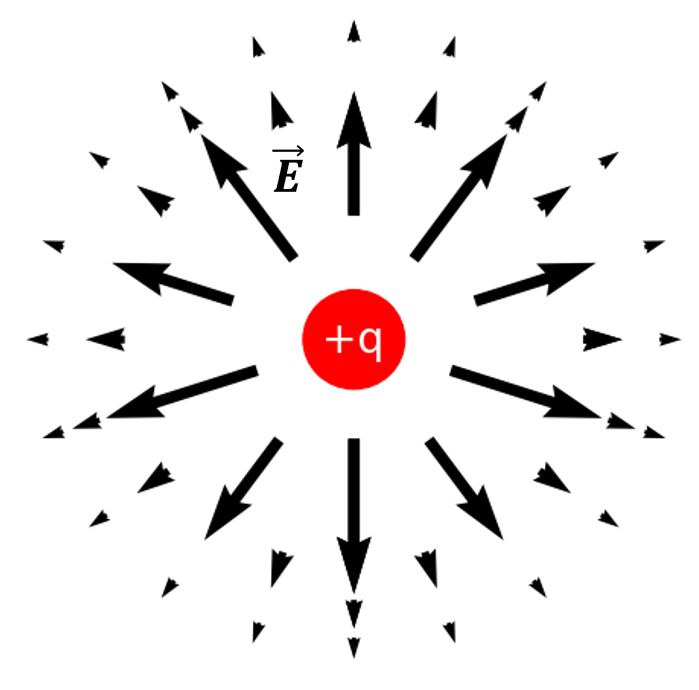
\includegraphics[width=0.3\linewidth]{files/1pos-bd746d90e839613ec799f32b8e33f122.png}
\caption[]{Electric field vectors near a point charge.}
\label{fig:ChargesFields:1pos}
\end{figure}

One disadvantage of visualizing a vector field with arrows is that the arrows take up space, and it can be challenging to visualize how the field changes magnitude and direction continuously through space. For this reason, one usually uses ``field lines'' to visualize a vector field. Field lines are continuous lines with the following properties:

\begin{itemize}
\item The direction of the vector field at some point in space is tangent to the field line at that point.
\item Field lines have a direction to indicate the direction of the field vector along the tangent (as there are two possibilities, parallel and anti-parallel).
\item The magnitude of the field is proportional to the density of field lines at that point. The more field lines near a location in space, the larger the magnitude of the field vector at that point.
\end{itemize}

An example of using field lines to represent a vector field in space is shown in Figure~\ref{fig:chargesfields:fieldlines}. The corresponding field vector is shown at two different positions in space ($A$ and $B$). At both positions, the vector is tangent to the field line at that position in space and points in the direction of the little arrow drawn at the end of the field lines. The field vector at point $A$ has a larger magnitude than the one at point $B$, since the field lines are more concentrated at point $A$ than at point $B$ (there are more field lines per unit area at that position in space, the field lines are closer together).

\begin{figure}[!htbp]
\centering
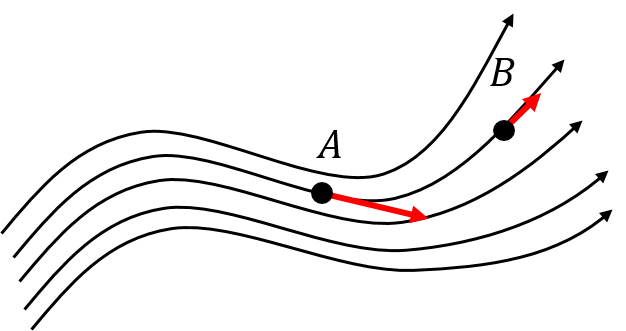
\includegraphics[width=0.4\linewidth]{files/fieldlines-3399c98223e3f2a01d954a6b769618be.png}
\caption[]{An example of determining a field vector from the continuous field lines.}
\label{fig:chargesfields:fieldlines}
\end{figure}

\begin{framed}
\textbf{Checkpoint:label: cp:chargesfields:efield}\\
It is possible for field lines to cross?\}

\begin{enumerate}
\item Yes.
\item No.
\end{enumerate}

\begin{framed}
\textbf{Answer}\\
\begin{enumerate}[resume]
\item
\end{enumerate}
\end{framed}
\end{framed}

Because the electric field vector always points in the direction of the force that would be exerted on a positive charge, electric field lines will point out from a positive charge and into a negative charge. The electric field lines for a combination of positive and negative charges is illustrated in Figure~\ref{fig:ChargesFields:2pos1neg}.

\begin{figure}[!htbp]
\centering
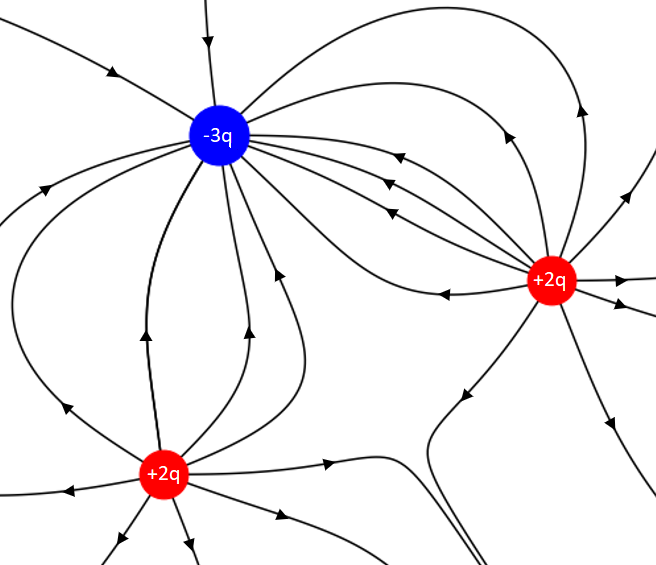
\includegraphics[width=0.5\linewidth]{files/2pos1neg-bb6e404661ee0b2000eae389bf928df8.png}
\caption[]{Field lines of two $+2q$ charges and one $-3q$ charge.}
\label{fig:ChargesFields:2pos1neg}
\end{figure}

\paragraph{Electric field from a charge distribution}

So far, we have only considered Coulomb's Law for point charges (charges that are infinitely small and can be considered to exist at a single point in space). We can use the principle of superposition to determine the electric field from a charged extended/continuous object by modelling that object as being made of many point charges. The electric field from that object is then the sum of the electric field from the point charges that make up that object.

Consider a charged wire that is bent into a semi-circle of radius $R$, as in Figure~\ref{fig:chargesfields:semicircle}. The wire carries a net positive electric charge, $+Q$, that is uniformly distributed along the length of the wire. We wish to determine the electric field vector at the centre of the circle.

\begin{figure}[!htbp]
\centering
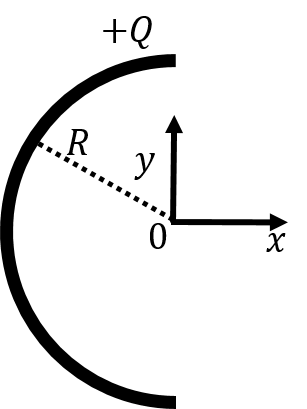
\includegraphics[width=0.2\linewidth]{files/semicircle-90ec0efe2d9da30eb5c806e6cf98e1f5.png}
\caption[]{A charged wire bent into a semi-circle of radius $R$.}
\label{fig:chargesfields:semicircle}
\end{figure}

We start by choosing a very small section of wire and model that section of wire as a point charge with infinitesimal charge $dq$ (as in Figure~\ref{fig:chargesfields:semicircle_sol}). A distance $R$ from that point charge, the electric field from that point charge will have magnitude, $dE$, given by:
\begin{equation}
dE=k\frac{dq}{R^2}
\end{equation}
The electric field vector, $d\vec E$, from the point charge $dq$ is illustrated in Figure~\ref{fig:chargesfields:semicircle_sol}.

\begin{figure}[!htbp]
\centering
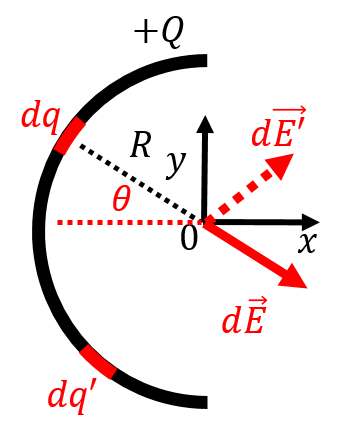
\includegraphics[width=0.2\linewidth]{files/semicircle_sol-cc72f82d349a967ff3aeacf8b69a4061.png}
\caption[]{Infinitesimal electric fields from point charges along the bent wire.}
\label{fig:chargesfields:semicircle_sol}
\end{figure}

Using the coordinate system that is shown, we define $\theta$ as the angle made by the vector from the origin to the point charge $dq$ and the $x$-axis. The electric field vector from $dq$ is then given by:
\begin{equation}
d\vec E = dE\cos\theta \hat x - dE\sin\theta \hat y
\end{equation}
The total electric field at the origin will be obtained by summing the electric fields from the different $dq$ over the entire semi-circle:
\begin{equation}
\vec E &= \int d\vec E = \int \left(dE\cos\theta \hat x - dE\sin\theta \hat y\right)\\
&=\left( \int dE\cos\theta \right)\hat x -\left( \int dE\sin\theta \right)\hat y\\
\therefore E_x &= \int dE\cos\theta\\
\therefore E_y &= -\int dE\sin\theta\\
\end{equation}
We are thus left with two integrals to solve for the $x$ and $y$ components of the electric field, respectively. Before jumping into solving the integrals, it is useful to think about the symmetry of the problem. Specifically, consider a second point charge, $dq'$, located symmetrically about the $x$-axis from charge $dq$, as illustrated in Figure~\ref{fig:chargesfields:semicircle_sol}. The charge $dq'$ will create a small electric field $d\vec E'$ as illustrated. When we add together $d\vec E$ and $d\vec E'$, the two $y$ components will cancel, and only the $x$ components will sum together. Similarly, for any $dq$ that we choose, there will always be another $dq'$ such that when we sum together their respective electric fields, the $y$ components will cancel. Thus, by symmetry, we can argue that the net $y$ component of the electric field, $E_y$, must be zero. We thus only need to evaluate the $x$ component of $\vec E$:
\begin{equation}
E_x = \int dE\cos\theta = \int k\frac{dq}{R^2} \cos\theta
\end{equation}
In order to solve this integral, we need to consider which variables change for different choices of the point charge $dq$. In this case, the distance $R$ is the same anywhere along the semi-circle, so only $\theta$ changes with different choices of $dq$, as $k$ is a constant. We can express $dq$ in terms of $d\theta$ and then use $\theta$ as the variable of integration (the variable that labels the different $dq$). $d\theta$ corresponds to a small change in the angle $\theta$, and is the angle that is subtended by the charge $dq$. That is, the charge $dq$ covers a small arc length, $ds$, of the semi-circle, which is related to $d\theta$ by:
\begin{equation}
ds = Rd\theta
\end{equation}
The total charge on the wire is given by $Q$, and the wire has a length $\pi R$ (half the circumference of a circle). Since the charge is distributed uniformly on the wire, the charge per unit length of any piece of wire must be constant. In particular, $dq$ divided by $ds$ must be equal to $Q$ divided by $\pi R$:
\begin{equation}
\frac{dq}{ds}&=\frac{Q}{\pi R}\\
\therefore dq &=\frac{Q}{\pi R}ds=\frac{Q}{\pi}d\theta
\end{equation}
where in the last equality we used the relation $ds=Rd\theta$. We now have all of the ingredients to solve the integral:
\begin{equation}
E_x &= \int k\frac{dq}{R^2} \cos\theta = \int_{-\pi/2}^{+\pi/2} k\frac{Q}{\pi R^2}\cos\theta d\theta\\
&= k\frac{Q}{\pi R^2}\int_{-\pi/2}^{+\pi/2}\cos\theta d\theta=k\frac{Q}{\pi R^2}\left[ \sin\theta \right]_{-\pi/2}^{+\pi/2}\\
&= k\frac{2Q}{\pi R^2}
\end{equation}
The total electric field vector at the centre of the circle is thus given by:
\begin{equation}
\vec E = k\frac{2Q}{\pi R^2} \hat x
\end{equation}
Note that if we had not realized that we did not need to solve the integral for the $y$ component, we would still find that it is zero:
\begin{equation}
E_y= -k\frac{Q}{\pi R^2}\int_{-\pi/2}^{+\pi/2}\cos\theta d\theta=-k\frac{Q}{\pi R^2}\left[ -\cos\theta \right]_{-\pi/2}^{+\pi/2}=0
\end{equation}

In order to determine the electric field at some point from any continuous charge distribution, the procedure is generally the same:

\begin{enumerate}
\item Make a \textit{good} diagram.
\item Choose a charge element $dq$.
\item Draw the electric field element, $d\vec E$, at the point of interest.
\item Write out the electric field element vector, $d\vec E$, in terms of $dq$ and any other relevant variables.
\item Think of symmetry: will any of the component of $d\vec E$ sum to zero over all of the $dq$?
\item Write the total electric field as the sum (integral) of the electric field elements.
\item Identify which variables change as one varies the $dq$ and choose an integration variable to express $dq$ and everything else in terms of that variable and other constants.
\item Do the sum (integral).
\end{enumerate}

\begin{framed}
\textbf{Olivia's Thoughts}\\
Before we get into the next few examples, I'm going to review the set-up for the  semi-circular wire, and explain why it's best to leave $dq$ in our expression as long as possible.

In this example, we were given a charged, semi-circular wire and asked to find the electric field. When asked to solve a new problem like this, many of us would start by trying to find a formula that applies to the problem. However, we were only given one formula for the electric field, $\vec E = k\frac{Q}{r^2}\hat r$, and this only applies to point charges. So, the only way that we can use this formula is to somehow make the semi-circular wire look like a bunch of point charges. To do this, we imagine that the wire looks like the left panel of Figure~\ref{fig:chargesfields:semicircle_redo}, where I have cut the wire into pieces, each of which has \textit{some} charge, $dq$.

\begin{figure}[!htbp]
\centering
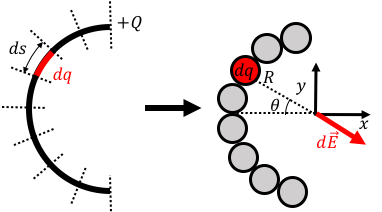
\includegraphics[width=0.6\linewidth]{files/semicircle_redo-1c8b776e96f2c9eeac1372ed73b9d871.png}
\caption[]{Left: Cutting up a wire with charge $Q$ into pieces with length $ds$ and charge $dq$. Right: Visualizing the semicircular wire as being made up of point charges.}
\label{fig:chargesfields:semicircle_redo}
\end{figure}

Since the pieces are very small, we can say that they are essentially point charges. Now, the problem looks something like the right panel of Figure~\ref{fig:chargesfields:semicircle_redo}, which we know how to solve. All we have to do is find the field from each point charge, $\vec E = k\frac{Q}{r^2}\hat r \rightarrow d\vec E = k\frac{dq}{r^2}\hat r$, and add them all up using an integral: $\vec E=\int d\vec E$. From the symmetry of the problem, we find that the $y$ contributions from the different point charges will cancel, so the  integral we need to solve is $E_x=\int k\frac{dq}{R^2}\cos\theta$.

Since $R$ and $k$ are constant, we just have to integrate over $\theta$. However, our integrand doesn't contain any $d\theta$ to integrate over. That's where our pal $dq$ comes in. Now that we know we want to integrate over $\theta$, we can \textit{choose} to express $dq$ in terms of $d\theta$. Looking back at the left panel of Figure~\ref{fig:chargesfields:semicircle_redo}, how much charge, $dq$, is in each piece? Well, $dq$ is just the charge of the whole wire, $Q$, divided by the length of the wire, $\pi R$, times the length of the piece, $ds$. Since each piece is in the shape of an arc, we can get $d\theta$ into this expression by using the formula for arc length, $ds=Rd\theta$. Therefore, $dq=(Q/\pi)( ds/R)=(Q/\pi)d\theta$, and we can now solve the integral.
\end{framed}

\begin{framed}
\textbf{Example 15.4}\\
A ring of radius $R$ carries a total charge $+Q$. Determine the electric field a distance $a$ from the centre of the ring, along the axis of symmetry of the ring.\}
In order to determine the electric field, we carry out the procedure outlined above, and start by drawing a good diagram, as in Figure~\ref{fig:chargesfields:ring}, showing: our coordinate system, our choice of $dq$, the electric field element vector $d\vec E$ that corresponds to $dq$, and variables ($r$, $\theta$) to specify the position of $dq$.

\begin{figure}[!htbp]
\centering
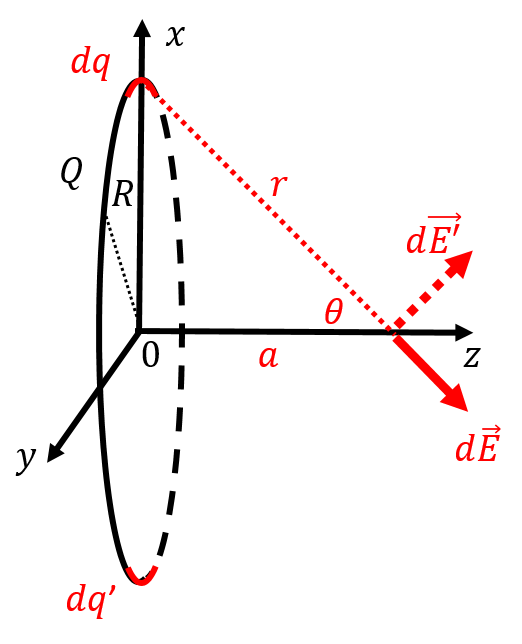
\includegraphics[width=0.3\linewidth]{files/ring-03c4e5297f14b48cab0838925852ec16.png}
\caption[]{Determining the electric field on the axis of a ring of radius $R$ carrying charge $Q$.}
\label{fig:chargesfields:ring}
\end{figure}

\begin{framed}
\textbf{Solution}\\
In this case, the figure is challenging to draw and visualize because of the three-dimensional nature of the problem. With the specific $dq$ that we chose, the electric field element vector is given by:
\begin{equation}
d\vec E = -dE\sin\theta \hat x + 0\hat y + dE\cos\theta \hat z
\end{equation}
where $d\vec E$ has magnitude:
\begin{equation}
dE = k\frac{dq}{r^2}
\end{equation}
The $x$ and $z$ components of the total electric field will then be given by:
\begin{equation}
E_x &= -\int dE\sin\theta=-\int k\frac{dq}{r^2}\sin\theta\\
E_z &= \int dE\cos\theta=\int k\frac{dq}{r^2}\cos\theta \\
\end{equation}
In general, if we had chosen a $dq$ that is not along one of the axes of the coordinate system, the electric field element vector would have components in all three directions. However, if we consider the symmetry of the ring, we can note that once we sum together all of the electric field elements, only the $z$ components will survive. Indeed, we have shown in Figure~\ref{fig:chargesfields:ring} that for each $dq$, there will be a $dq'$ located on the opposite side of the ring that will create an electric field element that will cancel all but the $z$ component of the field element from $dq$. We thus only need to consider the $z$ components of the electric field elements when determining the total electric field:
\begin{equation}
\vec E = E_z\hat z
\end{equation}
We now have to evaluate the integral for the $z$ component of the electric field:
\begin{equation}
E_z &= \int k\frac{dq}{r^2}\cos\theta \\
\end{equation}
and determine which quantities change as we move $dq$ around the ring. In this case, both $r^2$ and $\cos\theta$ are the same for all elements on the ring, and the integral is trivial:
\begin{equation}
E_z &= k\frac{1}{r^2}\cos\theta\int dq=k\frac{Q}{r^2}\cos\theta=kQ\frac{a}{(R^2+a^2)^\frac{3}{2}}  \\
\end{equation}
where the integral $\int dq$ simply means ``sum all of the charges $dq$ together'', which is equal to $Q$, the total charge on the ring.
In the last equality, we replaced $\cos\theta$ with the variables $a$ and $R$ that are provided in the question.
\end{framed}
\end{framed}

\begin{framed}
\textbf{Olivia's Thoughts}\\
In this example, we saw why it's best to leave $dq$ in our expression until we are ready to integrate. In this case, because $r$ and $\theta$ were both constant, it was not useful to write $dq$ in terms of another variable.
\end{framed}

\begin{framed}
\textbf{Example 15.5}\\
You have rubbed a glass rod with a silk cloth such that the glass rod has acquired a positive charge. The rod has a length, $L$, a negligible cross-section, and has acquired a total positive charge, $+Q$, that is uniformly distributed along the length of the rod. What is the electric field a distance $R$ from the centre of the rod?

\begin{framed}
\textbf{Solution}\\
In order to determine the electric field, we carry out the procedure outlined above, and start by drawing a good diagram, as in Figure~\ref{fig:chargesfields:finiteline}, showing: our coordinate system, our choice of $dq$ at a distance $y$ above the centre of the rod, the electric field element vector $d\vec E$ that corresponds to $dq$, and variables ($y$, $r$, $\theta$) to specify the position of $dq$.

\begin{figure}[!htbp]
\centering
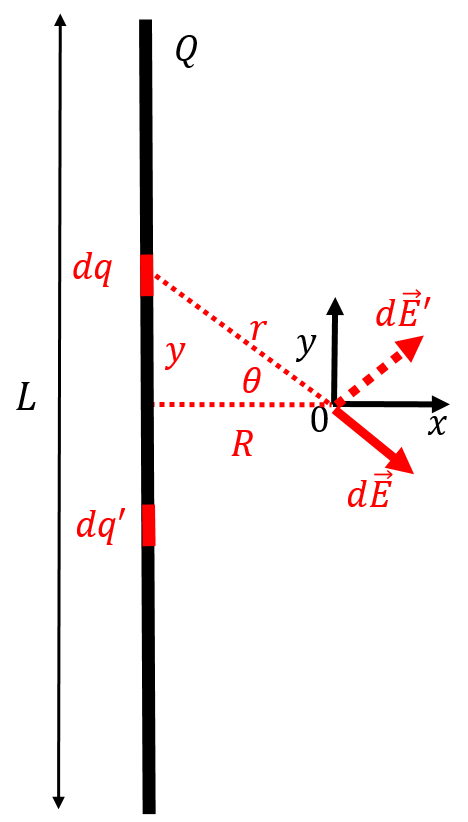
\includegraphics[width=0.3\linewidth]{files/finiteline-4685490417c1a722b87b010361357eb7.png}
\caption[]{Determining the electric field a distance $R$ from the centre of a rod of length $L$ carrying charge $Q$.}
\label{fig:chargesfields:finiteline}
\end{figure}

We define the origin to be located at the point where we want to determine the electric field, and the angle $\theta$ to be the angle between the horizontal and the position vector of $dq$. We can write the electric field element vector as:
\begin{equation}
d\vec E = dE\cos\theta \hat x - dE\sin\theta \hat y
\end{equation}
where $d\vec E$ has magnitude:
\begin{equation}
dE = k\frac{dq}{r^2}
\end{equation}
The $x$ and $y$ components of the total electric field will then be given by:
\begin{equation}
E_x &= \int dE\cos\theta=\int k\frac{dq}{r^2}\cos\theta \\
E_y &= -\int dE\sin\theta=-\int k\frac{dq}{r^2}\sin\theta\\
\end{equation}
Again, before proceeding with the integrals, we consider symmetry. Specifically, if we consider a charge $dq'$ located symmetrically about the $x$ axis from $dq$ (as illustrated in Figure~\ref{fig:chargesfields:finiteline}), we see that the $y$ component of the electric field element $d\vec E'$ that it creates will cancel the $y$ component of $d\vec E$. For each choice of $dq$, there will exist a corresponding choice $dq'$ which will result in the $y$ component of the net electric field being zero. We thus only need to evaluate the $x$ component of the total electric field:
\begin{equation}
\vec E = E_x \hat x = \left(\int k\frac{dq}{r^2}\cos\theta\right) \hat x
\end{equation}
Within the integrand, both $r$ and $\theta$ will change as we sum over the different charges $dq$ along the rod. A straightforward option to write the integral is to use $y$ as the integration constant, and to write $dq$, $r$, and $\cos\theta$ in terms of $y$. The charge $dq$ covers an infinitesimal length of the rod, $dy$. Since the rod is uniformly charged, the charge per unit length must be the same over a small length $dy$ as it is over the whole length of the rod:
\begin{equation}
\frac{dq}{dy}&=\frac{Q}{L}\\
\therefore dq &= \frac{Q}{L} dy
\end{equation}
It is often useful to introduce a constant charge per unit length, $\lambda=\frac{Q}{L}$, so that we can write the charge $dq$ as:
\begin{equation}
dq = \lambda dy
\end{equation}
We can also express $r^2$ and $\cos\theta$ in terms of $y$ (and $R$, which is constant):
\begin{equation}
r^2 &= y^2+R^2\\
\cos\theta&=\frac{R}{r}=\frac{R}{\sqrt{y^2+R^2}}
\end{equation}
Finally, we can combine this all into an integral that we can evaluate:
\begin{equation}
 E_x &= \int k\frac{dq}{r^2}\cos\theta\\
 &= k\int_{-L/2}^{L/2} \lambda \frac{1}{y^2+R^2}\frac{R}{\sqrt{y^2+R^2}} dy\\
 &= kR\lambda\int_{-L/2}^{L/2} \frac{1}{(y^2+R^2)^{\frac{3}{2}}} dy\\
 &= kR\lambda \left[  \frac{y}{R^2\sqrt{y^2+R^2}}\right]_{-L/2}^{L/2}\\
 \therefore E_x &= \frac{k\lambda}{R}\frac{L}{\sqrt{\left(\frac{L}{2}\right)^2+R^2}}
\end{equation}
If the rod were infinitely long (or very long compared to the distance $R$), the electric field becomes:
\begin{equation}
\lim_{L\to\infty}E_x=\frac{2k\lambda}{R}
\end{equation}
By using the charge per unit length, $\lambda$, we were able to easily generalize our result to that expected for an infinitely long rod with uniform charge density.

Solving the integral above in terms of the integration variable $y$ is difficult without some knowledge of integrals. For this specific integral, the easiest method to use from calculus is ``trig substitution''. We show below how we can arrive at a much easier integral if we had instead chosen the angle $\theta$ as the integration variable instead of $y$, and we will see that this is a physical illustration of the ``trig substitution method'' from calculus!

We go back to step 7 in our procedure and choose $\theta$ (instead of $y$) as the integration variable for the integral:
\begin{equation}
E_x &=\int k\frac{dq}{r^2}\cos\theta\\
\end{equation}
That is, we need to express $1/r^2$ and $dq$ in terms of $\theta$. To do this, we refer back to Figure~\ref{fig:chargesfields:finiteline}. Starting with $1/r^2$, we get:
\begin{equation}
r &= \frac{R}{\cos\theta}\\
\therefore \frac{1}{r^2}&=\frac{\cos^2\theta}{R^2}\\
\end{equation}
Now we need to find an expression for $dq$. We know that $dq=\lambda dy$, and $\lambda$ is just a constant, so we need to find $dy$ as a function of $\theta$:
\begin{equation}
y &= R\tan\theta\\
\therefore dy &= \frac{dy}{d\theta}d\theta=\frac{R}{\cos^2\theta}d\theta\\
\therefore dq &= \lambda dy =\lambda\frac{R}{\cos^2\theta}d\theta
\end{equation}
where in the second line, we took the derivative of $y=R\tan\theta$ with respect to $\theta$. With these expressions for $1/r^2$ and $dq$, the integral becomes trivial:
\begin{equation}
 E_x &= \int k\frac{dq}{r^2}\cos\theta\\
 &= k \int_{-\theta_0}^{\theta_0} \lambda\frac{R}{\cos^2\theta} \frac{\cos^2\theta}{R^2} \cos\theta d\theta\\
 &=\frac{k\lambda}{R}\int_{-\theta_0}^{\theta_0}\cos\theta d\theta\\
 &=\frac{k\lambda}{R}\left[\sin\theta \right]_{-\theta_0}^{\theta_0}\\
 &= \frac{2k\lambda}{R}\sin\theta_0
\end{equation}
where $\theta_0$ is the angle subtended by half of the rod. Referring to Figure~\ref{fig:chargesfields:finiteline}, we can easily see that:
\begin{equation}
\sin\theta_0=\frac{L/2}{\sqrt{\left(\frac{L}{2}\right)^2+R^2}}
\end{equation}
So that the total electric field is given by:
\begin{equation}
E_x &=\frac{2k\lambda}{R}\sin\theta_0=\frac{k\lambda}{R}\frac{L}{\sqrt{\left(\frac{L}{2}\right)^2+R^2}}
\end{equation}
as found before. Furthermore, in the limit of an infinitely long rod, the angle $\theta_0$ tends to $\frac{\pi}{2}$, so that the electric field becomes:
\begin{equation}
E_x=\lim_{\theta_0\to\frac{\pi}{2}}\frac{2k\lambda}{R}\sin\theta_0=\frac{2k\lambda}{R}
\end{equation}
\textbf{Discussion:} In this example, we saw how to apply the principle of superposition to determine the electric field near a finite and a infinite line of charge with constant charge per unit length. We showed that it was relatively straightforward to set up the integral in terms of $dy$, but not so easy to solve the integral. We then showed that by using $\theta$ as the integration variable, we could arrive at a much easier integral. This change of variable corresponds to a physical variable in our problem, but is also the basis for the more abstract ``trig substitution'' method used to solve integrals in calculus.
\end{framed}
\end{framed}

\begin{framed}
\textbf{Example 15.6}\\
Calculate the electric field a distance, $a$, above a infinite plane that carries uniform charge per unit area, $\sigma$.\}
In this case, we need to determine the field above an object that is two dimensional (a plane). In the previous examples (a ring, a line of charge), we modelled a one dimensional object (e.g. the line), as being made of many point charges (0-dimensional objects). We treated those point charges has having an infinitesimal length along the object so that we could sum them together to obtain the object (e.g. $dy$ was the length of the charge for the rod/line of charge).

\begin{framed}
\textbf{Solution}\\
In order to model the two-dimensional object (the plane), we model it has being the sum of many one dimensional objects. We can model a plane either as a rectangle of width, $W$, and length, $L$, as shown in the left panel of Figure~\ref{fig:chargesfields:planecharge} or as a disk of radius, $R$, as shown in the right panel. To model an infinite plane, we can then take the limit of either $L$ and $W$ going to infinity (rectangle), or of $R$ going to infinity (disk). We can model the rectangle as being the sum of many lines of \textbf{finite} length, $L$, and infinitesimal width, $dx$. Similarly, we can model the disk as the sum of infinitesimally thin rings of \textbf{finite} radius, $r$, and thickness, $dr$. In both cases, we know how to model the field from a line of charge (Example~15.5) or from a ring (Example~15.4).

\begin{figure}[!htbp]
\centering
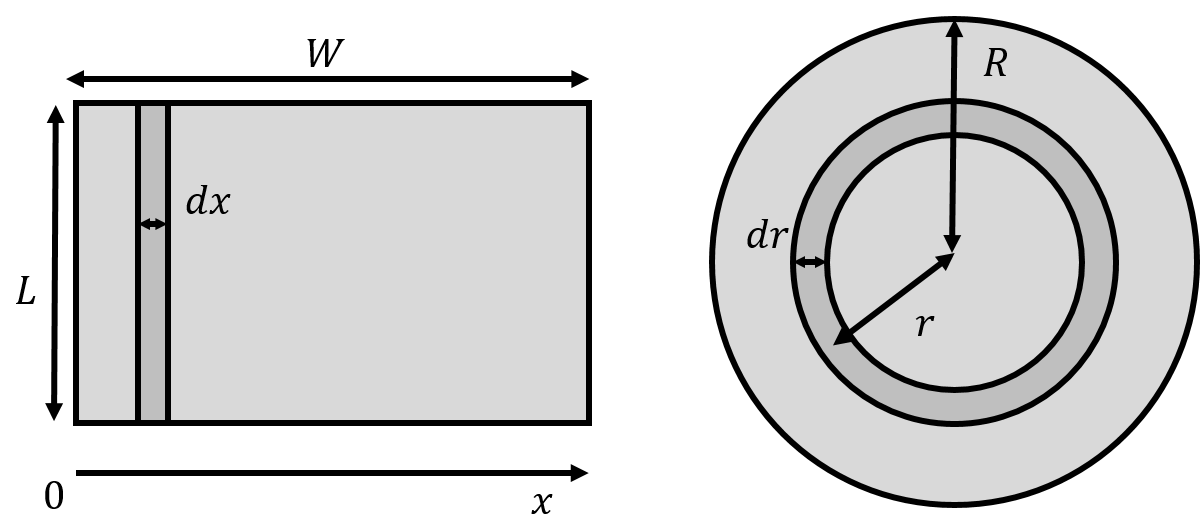
\includegraphics[width=0.7\linewidth]{files/planecharge-ef931468f92f58cf31fa48dcf255be7e.png}
\caption[]{A two-dimensional object such as a plane modelled as a the sum of infinitely thin lines (left panel) or as the sum of infinitely thin rings (right panel).}
\label{fig:chargesfields:planecharge}
\end{figure}

We proceed by modelling the plane as a disk made up of infinitesimal rings. Our infinitesimal charge, $dq$, is thus the charge on a ring of radius $r$ and thickness $dr$, as illustrated in Figure~\ref{fig:chargesfields:disk}.

\begin{figure}[!htbp]
\centering
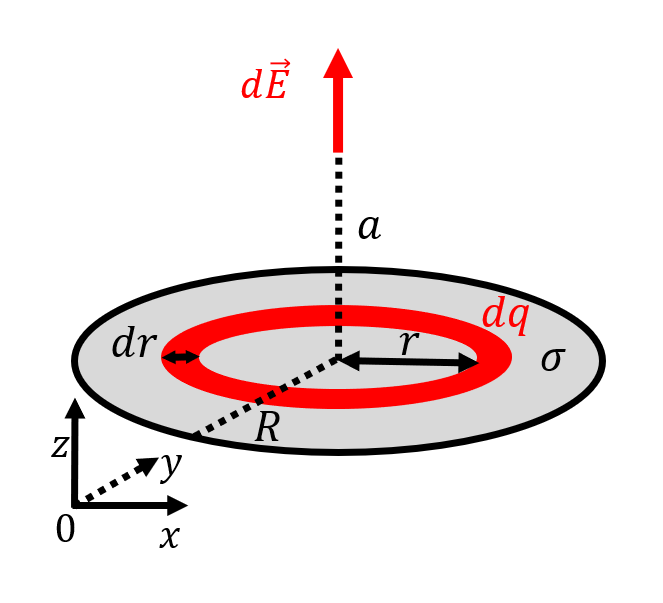
\includegraphics[width=0.3\linewidth]{files/disk-725ab7b22a1889b37e3080521f570aa5.png}
\caption[]{Modelling the field from a disk as the sum of fields from concentric thin rings.}
\label{fig:chargesfields:disk}
\end{figure}

We know from Determining~the~electric~field~on~the~axis~of~a~ring~of~radius~R~carrying~charge~Q. that the magnitude of the electric field a distance $a$ from the centre of the ring, along its axis of symmetry (the $z$ axis in Figure~\ref{fig:chargesfields:disk}), is given by:
\begin{equation}
dE = kdq\frac{a}{(r^2+a^2)^\frac{3}{2}}
\end{equation}
By symmetry, for all of the different infinitesimal rings that make up the disk, the field will always point along the $z$ axis. In order to determine the total field, we sum (integrate) the values of $dE$, over all of the rings, from a radius of $r=0$ to a radius $r=R$. For each ring, the value of $r$ will be different, so we need to express $dq$ in terms of $dr$ in order to perform the integral. We know that the plane has a uniform charge per unit area given by $\sigma$. The charge $dq$ of an infinitesimal ring is given by:
\begin{equation}
dq = \sigma dA=\sigma 2\pi r dr
\end{equation}
where $dA=2\pi r dr$ is the area of the infinitesimal ring of radius $r$ and thickness $dr$ (think of unfolding the ring into a rectangle of height $dr$ and length $2\pi r$, the circumference of the circle, in order to determine the area). We now have all of the ingredients in order to determine the total electric field:
\begin{equation}
E &= \int dE = \int_0^R kdq\frac{a}{(r^2+a^2)^\frac{3}{2}}  = 2\pi k a \sigma \int_0^R \frac{r}{(r^2+a^2)^\frac{3}{2}}dr\\
&=2\pi k a \sigma \left[  \frac{-1}{\sqrt{r^2+a^2}}\right]_0^R=2\pi k  \sigma\left(1-\frac{a}{R^2+a^2} \right)
\end{equation}
Finally, we can take the limit of $R\to\infty$ in order to get the electric field above an infinite plane:
\begin{equation}
E=\lim_{R\to\infty}2\pi k  \sigma\left(1-\frac{a}{R^2+a^2} \right)=2\pi k\sigma=\frac{\sigma}{2\epsilon_0}
\end{equation}
where we used $\epsilon_0$ in the last equality as the result is a little cleaner without the factors of $\pi$. Note that for an infinite plane of charge, the electric field does not depend on the distance (our variable $a$) from the plane!

\textbf{Discussion:} In this example, we showed how we can model a two-dimensional charge distribution as the sum of one-dimensional charge distributions. In particular, we showed that an infinite plane of charge can be modelled as the sum of many lines charges or of many rings of charge (we chose the latter in the above). We also found that the electric field above an infinite plane of charge does not depend on the distance from the plane; that is, the electric field is constant above an infinite plane of charge.
\end{framed}
\end{framed}

\begin{framed}
\textbf{Josh's Thoughts}\\
A common source of confusion is the process of solving for the electric field produced by continuous charges. Point charges are well defined in space as being entirely contained within a single point, while continuous charges are objects which occupy 1, 2, or 3 dimensions. The electric field produced by point charges are easily modelled by $\vec E = \frac{kQ}{r^2}\hat r$, but the electric fields produced by continuous charges must usually be obtained from an integral.

When a charge is distributed, the charge on the object must be broken down into many small charges which are written as $dq$. From there, $dq$ is rewritten in terms of a position variable over which it is convenient to integrate. Think of the position variable as a variable that you can use to distinguish charges, $dq$, located at different positions along the object.

For example, referring to Figure~\ref{fig:chargesfields:rodexample}, if I wanted to determine $E$ at the top of a rod (left-hand panel), it would be most convenient for me to integrate over $x$, but if I wanted to determine $E$ on the side of a rod, it would be most convenient to integrate over $\theta$.

\begin{figure}[!htbp]
\centering
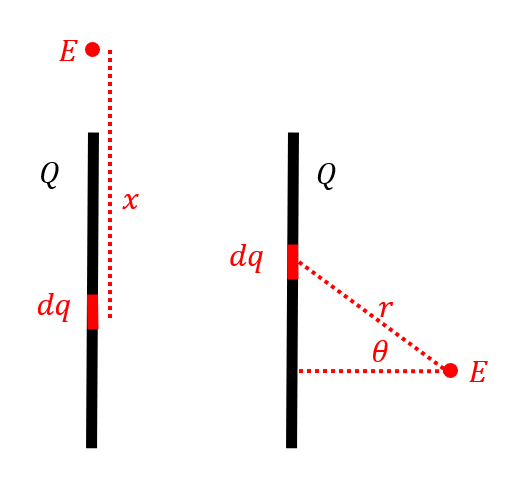
\includegraphics[width=0.4\linewidth]{files/rodexample-76239b7407f7a41e29db62973439260f.png}
\caption[]{Calculating the electric field produced by a rod at different positions.}
\label{fig:chargesfields:rodexample}
\end{figure}

In order to determine the bounds of the integral, think of the range in position variable that is required in order to cover the entire object. I recommend paying close attention to Example~15.4, Example~15.5, and Example~15.6, and attempting questions which require integration on the Question Library.
\end{framed}

\subsubsection{The electric dipole}\label{sec:chargesfields:electricdipole}

Electric dipoles are a specific combination of a positive charge $+Q$ held at a fixed distance, $l$, from an equal and opposite charge, $-Q$, as illustrated in Figure~\ref{fig:chargesfields:dipole}.

\begin{figure}[!htbp]
\centering
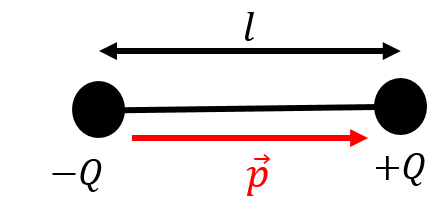
\includegraphics[width=0.3\linewidth]{files/dipole-46c3107dc981a624ca87141b9e165fa2.png}
\caption[]{An electric dipole and its corresponding dipole vector, $\vec p$.}
\label{fig:chargesfields:dipole}
\end{figure}

Dipoles can be represented by their ``electric dipole vector'' (or ``electric dipole moment''), $\vec p$, defined to point in the direction \textbf{from the negative charge to the positive charge}, with magnitude:
\begin{equation}
p=Ql
\end{equation}
Dipoles arise frequently in nature. For example, a water molecule can be modelled as a dipole. In a water molecule, the two hydrogen atoms are not symmetrically arranged around the oxygen atom. The electrons tend to stay closer to the oxygen atom, so the oxygen atom has an excess of 2 electrons, while each proton has a deficit of 1 electron. This results in a separation of charge (polarization), which can be modelled as an electric dipole, as in Figure~\ref{fig:chargesfields:h20}.

\begin{figure}[!htbp]
\centering
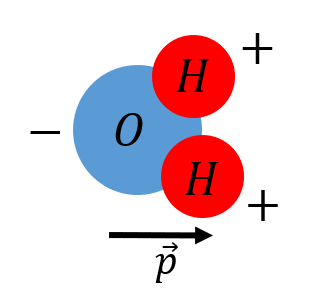
\includegraphics[width=0.2\linewidth]{files/h20-c9e951e5ea9119ebb1b2a21e09add397.png}
\caption[]{A water molecule can be modelled as an electric dipole.}
\label{fig:chargesfields:h20}
\end{figure}

When a dipole is immersed in a uniform electric field, as illustrated in Figure~\ref{fig:chargesfields:dipoleinfield}, the net force on the dipole is zero because the force on the positive charge will always be equal to and in the opposite direction of the force on the negative charge.

\begin{figure}[!htbp]
\centering
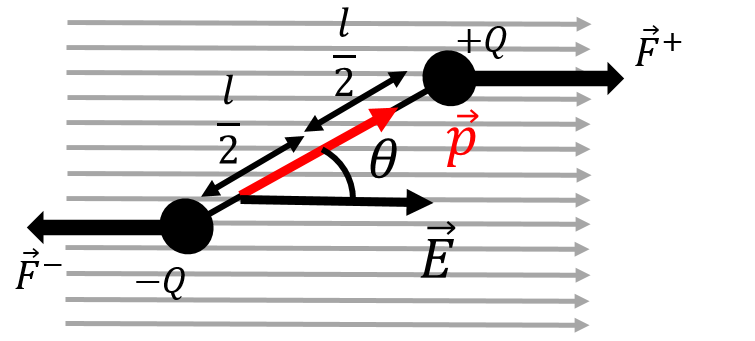
\includegraphics[width=0.6\linewidth]{files/dipoleinfield-89cb18f52c976098c978acd723095b35.png}
\caption[]{An electric dipole in a uniform electric field.}
\label{fig:chargesfields:dipoleinfield}
\end{figure}

Although the net force on the dipole is zero, there is still a net torque about its centre that will cause the dipole to rotate (unless the dipole vector is already parallel to the electric field vector). If the dipole vector makes an angle, $\theta$, with the electric field vector (as in Figure~\ref{fig:chargesfields:dipoleinfield}), the magnitude of the net torque on the dipole about an axis perpendicular to the page and through the centre of the dipole is given by:
\begin{equation}
\tau&=\frac{l}{2}F^+\sin\theta+\frac{l}{2}F^-\sin\theta\\
&=\frac{l}{2}QE\sin\theta+\frac{l}{2}QE\sin\theta\\
&=QlE\sin\theta\\
\tau&=pE\sin\theta
\end{equation}
In Figure~\ref{fig:chargesfields:dipoleinfield}, the torque vector is into the page (the forces will make it rotate clockwise), which is the same direction as the cross product, $\vec p \times \vec E$. Note that the magnitude of the torque is also equal to the magnitude of the cross product. Thus, in general, the torque vector on a dipole, $\vec p$, from an electric field, $\vec E$, is given by:
\begin{equation}
\boxed{\vec \tau =\vec p \times \vec E}
\end{equation}
In particular, note that the torque is zero when the dipole and electric field vectors are parallel. Thus, a dipole will always experience a torque that tends to align it with the electric field vector. The dipole is thus in a stable equilibrium when it is parallel to the electric field.

\begin{framed}
\textbf{Checkpoint:label: cp:chargesfields:efield}\\
When an electric dipole is such that its dipole vector is anti-parallel to the electric field vector, the dipole is

\begin{enumerate}
\item not in equilibrium.
\item in a stable equilibrium.
\item in an unstable equilibrium.
\end{enumerate}

\begin{framed}
\textbf{Answer}\\
\begin{enumerate}[resume]
\item
\end{enumerate}
\end{framed}
\end{framed}

We can also model the behaviour of the dipole using energy. If a dipole is rotated away from its equilibrium orientation and then released, it will gain (rotational) kinetic energy as it tries to return to equilibrium, and will oscillate about the equilibrium position. When the dipole is held out of equilibrium, we can think of it has having potential energy. To determine the functional form of that potential energy function, we consider the work done in rotating the dipole from an angle $\theta_1$ to an angle $\theta_2$ (where the angle is between the dipole and the electric field vectors):
\begin{equation}
W&=\int_{\theta_1}^{\theta_2} \tau d\theta=\int_{\theta_1}^{\theta_2} -pE\sin\theta d\theta=-pE\int_{\theta_1}^{\theta_2} \sin\theta d\theta\\
&=pE[\cos\theta]_{\theta_1}^{\theta_2}=pE\cos\theta_2-pE\cos\theta_1
\end{equation}
where the negative sign in the torque is to indicate that the torque is in the opposite direction from increasing $\theta$ (in Figure~\ref{fig:chargesfields:dipoleinfield}, the torque is clockwise whereas the angle $\theta$ increases counter-clockwise). The net work done in going from position $\theta_1$ to $\theta_2$ is the negative of the change in potential energy in going from $\theta_1$ to $\theta_2$. Thus, we define the potential energy of an electric dipole, $\vec p$, in an electric field, $\vec E$, as:
\begin{equation}
\boxed{U=-pE\cos\theta=-\vec p\cdot \vec E}
\end{equation}
which has a negative sign, and we also recognize that this is equivalent to the scalar product between $\vec p$ and $\vec E$. Note that the negative sign makes sense because systems experience a force/torque that will decrease their potential energy. When the angle is zero, $\cos\theta=1$, is maximal. Since we need the position with $\theta=0$ to have the lowest potential energy, the minus sign guarantees that all values of $\theta$ other than zero will give a potential energy that is higher (greater than) $( -1) pE$. Remember that only changes in potential energy are relevant, so the minus sign should not bother you, although you should think about whether it makes sense.

\subsubsection{Summary}

Objects can acquire a net charge if they acquire a net excess or deficit of electrons. Charges are never created, they are only transferred from one object to another. One can charge an object by friction, conduction, or induction. Materials can be classified broadly as conductors, where electrons can move freely in a material, or insulators, in which electrons remain tightly bound to the atoms in the material. If a conducting object acquires a net charge, those charges will migrate to the surface of the conductor.

Coulomb was the first to quantitatively describe the electric force exerted on a point charge, $Q_1$, by a second point charge, $Q_2$, located a distance, $r$, away:
\begin{equation}
\vec F_{12}=k\frac{Q_1Q_2}{r^2}\hat r_{21}=\frac{1}{4\pi\epsilon_0}\frac{Q_1Q_2}{r^2}\hat r_{21}
\end{equation}
where $\hat r_{21}$ is the unit vector from  $Q_2$ to $Q_1$. One can write the force using either Coulomb's constant, $k$, or the permittivity of free space, $\epsilon_0$. Coulomb's force is attractive if the product $Q_1Q_2$ is negative, and repulsive if the product is positive. Thus, charges of the same sign exert a repulsive force on each other, whereas opposite charges exert an attractive force on each other.

Mathematically, Coulomb's Law is identical to the gravitational force in Newton's Universal Theory of Gravity, which implies that it is conservative. The electric field vector at some position in space is defined to be the electric force per unit charge at that position in space. That is, at some position in space where the electric field vector is $\vec E$, a charge, $q$, will experience an electric force:
\begin{equation}
\vec F=q\vec E
\end{equation}
much like a mass, $m$, will experience a gravitational force, $m\vec g$, in a position in space where the gravitational field is $\vec g$. A positive charge will experience a force in the same direction as the electric field, whereas a negative charge will experience a force in the direction opposite of the electric field. The electric field at position, $\vec r$, from a point charge, $Q$, located at the origin, is given by:
\begin{equation}
\vec E = k\frac{Q}{r^2}\hat r
\end{equation}
One can visualize an electric field by using ``field lines''. The field vector at any point in space has a magnitude that is proportional to the number of field lines at that point, and a direction that is tangent to the field lines at that point.

We can model the electric field from a continuous charged object (i.e. not a point charge) by modelling the object as being made up of many point charges. Often, it is easiest to model an $N$-dimensional object as being the sum of objects of dimension $N -1$ and an infinitesimal length in the remaining dimension. For example, we modelled a line of charge as the sum of point charges that have an infinitesimal length, and we modelled a disk of charge as the the sum of rings that have an infinitesimal thickness. In general, the strategy to model the electric field from a continuous distribution of charge is the same:

\begin{enumerate}
\item Make a \textit{good} diagram.
\item Choose a charge element $dq$.
\item Draw the electric field element, $d\vec E$, at the point of interest.
\item Write out the electric field element vector, $d\vec E$, in terms of $dq$ and any other relevant variables.
\item Think of symmetry: will any of the component of $d\vec E$ sum to zero over all of the $dq$?
\item Write the total electric field as the sum (integral) of the electric field elements.
\item Identify which variables change as one varies the $dq$ and choose an integration variable to express $dq$ and everything else in terms of that variable and other constants.
\item Do the sum (integral).
\end{enumerate}

Finally, we introduced the electric dipole, which is an object comprised of two equal and opposite charges, $+Q$ and $-Q$, held at fixed distance, $l$, from each other. One can model an electric dipole using its dipole vector, $\vec p$, defined to point in the direction from $-Q$ to $+Q$, with magnitude:
\begin{equation}
p=Ql
\end{equation}
When a dipole is immersed in a uniform electric field, $\vec E$, it will experience a torque given by:
\begin{equation}
\vec\tau=\vec p\times \vec E
\end{equation}
The torque will act such as to align the vector $\vec p$ with the electric field vector. We can define a potential energy, $U$, to model the energy that is stored in a dipole when it is not aligned with the electric field:
\begin{equation}
U=-\vec p \cdot \vec E
\end{equation}
The point of lowest potential energy corresponds to the case when $\vec p$ and $\vec E$ are parallel, whereas the point of highest potential energy is when the two vectors are anti-parallel.

\begin{framed}
\textbf{Important Equations}\\
\textbf{Coulomb's Law:}
\begin{equation}
\vec F_{12}=k\frac{Q_1Q_2}{r^2}\hat r_{21}=\frac{1}{4\pi\epsilon_0}\frac{Q_1Q_2}{r^2}\hat r_{21}
\end{equation}
\textbf{Electric field:}
\begin{equation}
\vec E = k \frac{Q}{r^2}\vec r \\
\vec E = \int d \vec E \\
\end{equation}
\textbf{Electric force:}
\begin{equation}
\vec F = q \vec E \\
\end{equation}

\textbf{Electric dipole moment:}
\begin{equation}
p = Ql \\
\end{equation}
\textbf{Torque on a dipole:}
\begin{equation}
\vec \tau = \vec p \times \vec E \\
\end{equation}
\textbf{Potential energy stored in a dipole:}
\begin{equation}
U = -\vec p \cdot \vec E \\
\end{equation}
\end{framed}

\begin{framed}
\textbf{Important Definitions}\\
\begin{itemize}
\item \textbf{Electric field:} The electric field is defined to be the electric force per unit charge. SI units: ${\rm \left[{N/C}, {\rm V/m}\right]}$. Common variable(s): $\vec E$.
\item \textbf{Coulomb's constant:} A fundamental physical constant which relates charge and distance to electric field. SI units: [ ${\rm Nm^2C^{ -2}}$]. Common variable(s): $k$.
\item \textbf{Electric dipole moment:} A vector used to represent an electric dipole. SI units: ${\rm \left[{Cm}\right]}$. Common variable(s): $\vec p$.
\item \textbf{Linear charge density:} The charge per unit length of an object. SI units: ${\rm \left[{C/m}\right]}$. Common variable(s): $\lambda$.
\item \textbf{Surface charge density:} The charge per unit area of an object. SI units: ${\rm \left[{Cm^{ -2}}\right]}$. Common variable(s): $\sigma$.
\item \textbf{Volume charge density:} The charge per unit volume of an object. SI units: ${\rm \left[{Cm^{ -3}}\right]}$. Common variable(s): $\rho$.
\end{itemize}
\end{framed}

\subsubsection{Thinking about the material}

\begin{framed}
\textbf{Reflect and research}\\
\begin{itemize}
\item Which molecule has the largest dipole moment? Why?
\item How does a laser printer exploit physical properties covered in this chapter?
\item How does a Van de Graff generator work?
\item On the 20th of May, 2019, SI base units were redefined. How does this affect Coulomb's constant?
\end{itemize}
\end{framed}

\begin{framed}
\textbf{To try at home}\\
\begin{itemize}
\item Rub your hands or feet along various household items to test their electron affinity. Which household items produce a static charge?
\item After charging your body, research the electron affinity of the surface you used to charge yourself. Knowing this, how many electrons were transferred while you charged yourself?
\end{itemize}
\end{framed}

\begin{framed}
\textbf{To try in the lab}\\
\begin{itemize}
\item Propose an experiment to measure the Coulomb's constant.
\item Propose an experiment to organize various materials based on their electron affinity.
\end{itemize}
\end{framed}

\subsubsection{Sample problems and solutions}

\paragraph{Problems}

\begin{framed}
\textbf{Problem 15.1}\\
Consider three charged rods of length $L$ which are arranged to form a triangle, as shown in Figure~\ref{fig:ChargesFields:trianglediagram}. If the charge on each rod is evenly distributed, what is the net electric field at the centre of the triangle (defined as the intersection of the bisectors)?

\begin{figure}[!htbp]
\centering
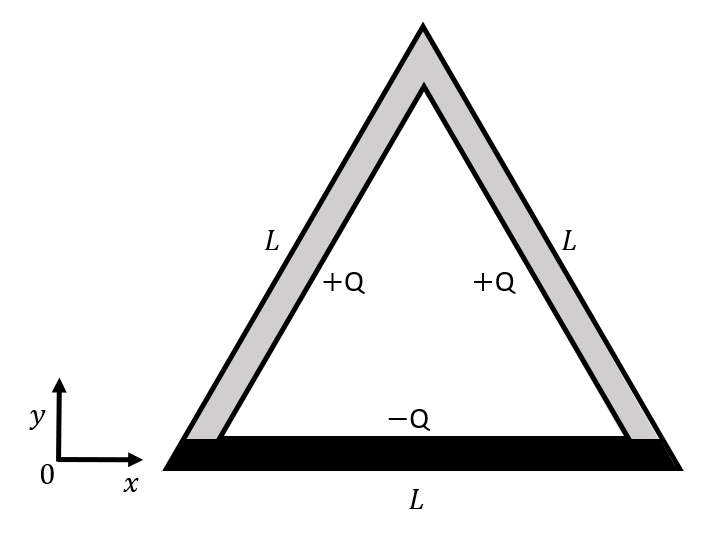
\includegraphics[width=0.4\linewidth]{files/trianglediagram-57cfb5fcb5af53ea4a1cdbd640dc0dee.png}
\caption[]{A triangle made up of charged rods}
\label{fig:ChargesFields:trianglediagram}
\end{figure}
\end{framed}

\begin{framed}
\textbf{Problem15.2}\\
Suppose that an electric dipole, with electric dipole moment, $\vec p$, is placed in a uniform electric field $\vec E$. In equilibrium, the dipole moment vector, $\vec p$, will be parallel to the electric field vector, $\vec E$. Show that, if the dipole is displaced (rotated) by a small angle away from the equilibrium, the dipole will then experience simple harmonic motion.
\end{framed}

\paragraph{Solutions}

\begin{framed}
\textbf{Solution 15.1}\\
We can model the object as the sum of three finite length wires of the length, $L$. In Example~15.5, we determined that the electric field produced at a distance, $R$, by a finite wire that subtends an angle $2\theta_0$ is given by:
\begin{equation}
E = \frac{2k\lambda}{R}\sin\theta_0
\end{equation}
The angle $\theta_0$ is easily found to be $\theta_0 = \frac{\pi}{3}$, as shown in Figure~\ref{fig:ChargesFields:trianglesolution}. The distance, $R$, is similarly found to be given by:
\begin{equation}
R = \frac{L}{2}\tan\left(\frac{\pi}{6}\right)=\frac{\sqrt{3}}{6}L
\end{equation}
\begin{figure}[!htbp]
\centering
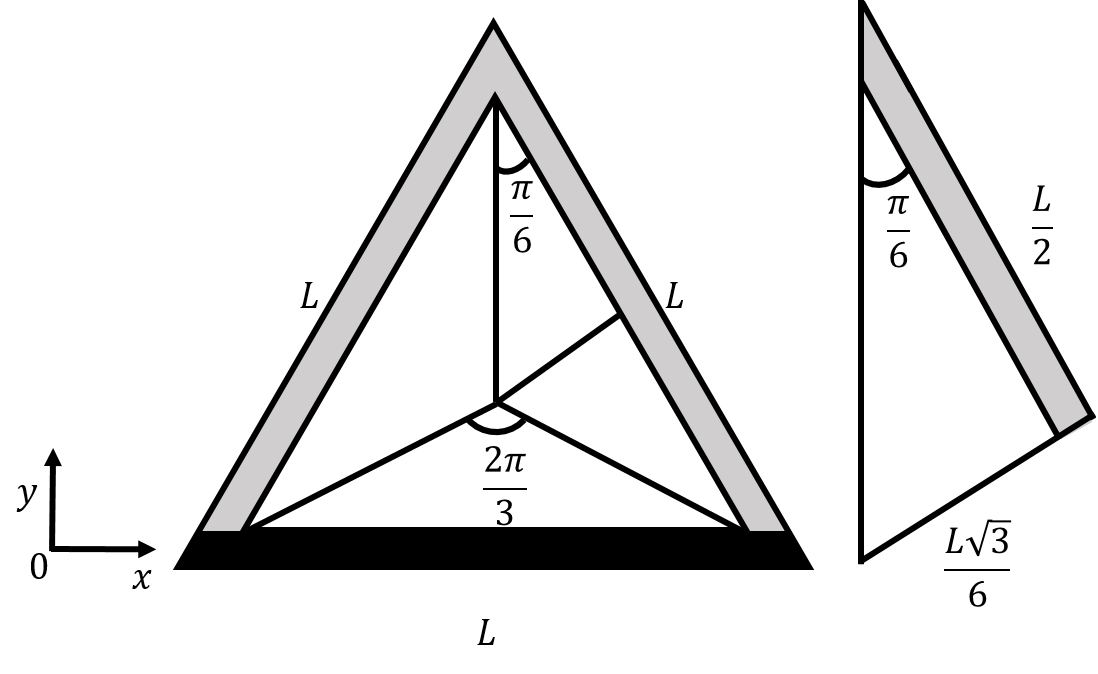
\includegraphics[width=0.6\linewidth]{files/trianglesolution-2125f2bf1c8dc2704b3068619355f64e.png}
\caption[]{Solving for $\theta_0$ and $R$}
\label{fig:ChargesFields:trianglesolution}
\end{figure}

Thus, the magnitude of the electric field from one wire is given by:
\begin{equation}
E&= \frac{2k\lambda}{R}\sin\left(\frac{\pi}{3}\right)=\frac{\sqrt{3}k\lambda}{R}=\frac{\sqrt{3}k\lambda}{\frac{\sqrt{3}}{6}L}=\frac{6k\lambda}{L}
\end{equation}
The charge, $Q$, is evenly distributed along the rod of length, $L$, so that we can rewrite the charge density as $\lambda=\frac{Q}{L}$, which gives:
\begin{equation}
E &= \frac{6k\lambda}{L} = \frac{6kQ}{L^2}
\end{equation}
This is the magnitude of the electric field produced by each side of the triangle. The two positive wires will produce electric fields whose horizontal components ($x$-axis in Figure~\ref{fig:ChargesFields:trianglesolution}) cancel. The net electric field from the two positive, $\vec E^{pos}$, wires will then be in the negative $y$ direction:
\begin{equation}
E_{y}^{pos}=-2 \left( \frac{6kQ}{L^2}  \right) \cos\left(\frac{\pi}{3} \right)=-\frac{6kQ}{L^2}
\end{equation}
The negative wire will also produce a field, $\vec E^{neg}$, in the negative $y$ direction (the only component of the field is in the $y$ direction):
\begin{equation}
E_{y}^{neg}=- \frac{6kQ}{L^2}
\end{equation}
Thus, the total field at the centre of the triangle, when (vectorially) adding the fields from the two positive wires and the negative wire is given by:
\begin{equation}
\vec E = \left(-\frac{6kQ}{L^2} - \frac{6kQ}{L^2} \right)\hat y=- \frac{12kQ}{L^2}\hat y
\end{equation}
\end{framed}

\begin{framed}
\textbf{Solution 15.2}\\
When the dipole is rotated from the equilibrium position by an angle $\theta$, it will experience a restoring torque exerted by the electric field, with magnitude:
\begin{equation}
\tau = -pE\sin\theta
\end{equation}
where we have inserted a minus sign to indicate that this is a restoring torque, in the opposite direction of increasing angle $\theta$. The net torque is then equal to the moment of inertia times the angular acceleration of the dipole (Newton's Second Law applied for rotation):
\begin{equation}
-pE\sin\theta &= I\alpha\\
\therefore \alpha &= -\frac{pE}{I}\sin\theta\sim-\frac{pE}{I}\theta
\end{equation}
where in the last equality, we made the small angle approximation ($\sin\theta\sim\theta$). This has the form for simple harmonic motion, with angular frequency, $\omega$:
\begin{equation}
\frac{d^2\theta}{dt^2}&=-\omega^2 \theta\\
\alpha=\omega &=\sqrt{\frac{pE}{I}}
\end{equation}
\end{framed}